% !TEX encoding = UTF-8 Unicode
%\documentclass[twoside]{article}
\documentclass[twocolumn,10pt]{article}
\usepackage[french]{babel}
\usepackage[utf8]{inputenc}
\usepackage[T1]{fontenc}

\usepackage{amsmath}
\usepackage{amssymb}
\usepackage{amsfonts}
\usepackage{graphicx}
% \usepackage{bbm}

\usepackage[margin=2cm,top=32mm,columnsep=20pt]{geometry}
\usepackage{multirow,multicol} % Style double colonne
\usepackage{abstract} % Customization de l'abstract
\usepackage{fancyhdr} % en-têtes et pieds de page
\usepackage{float} % Nécessaire pour les tables et figures dans l'environnement double colonne

\usepackage[colorlinks=true,linkcolor=red,urlcolor=blue,filecolor=green]{hyperref} % hyperliens
% \usepackage{dtk-logos}

% En-têtes et pieds de page
\pagestyle{fancy}
\fancyhead{} % Blank out the default header
\fancyfoot{} % Blank out the default footer
\fancyfoot[RO,LE]{\thepage} % Custom footer text

\setlength{\parskip}{1ex} % espace entre paragraphes

\newcommand{\bsx}{\boldsymbol{x}}
\newcommand{\bsX}{\boldsymbol{X}}
\newcommand{\transp}[1]{{#1}^\top}
\usepackage[
    backend=biber,
    style=alphabetic,
    citestyle=numeric,
    style=numeric
]{biblatex}
\addbibresource{bibliographie.bib}
\usepackage[nottoc,numbib]{tocbibind}

% Affichage du code python
% \usepackage[cachedir=cache/minted-\jobname]{minted}
% \setminted{encoding=utf8, numbersep=3pt, xleftmargin={2em}, breaklines, linenos=true}
% \def\Rcode#1{\mintinline{R}{#1}}
% \def\pycode#1{\mintinline{python}{#1}}


%----------------------------------------------------------------------------------------

\title{Projet SY09}

\author{
    Julia CAVICCHI\
    \and
    Bilel DEBBABI\
    \and
    Pierre ROMON\
}
\date{\today}

\begin{document}

\maketitle % Insert title
\thispagestyle{fancy} % All pages have headers and footers


\section{Introduction}

Dans le cadre du projet de SY09 nous avons été amenés à analyser un jeu de données portant sur les caractéristiques biomécaniques de patients orthopédiques. Nous nous sommes attachés à en extraire les informations pertinentes afin de détecter chez un patient pour lequel on connaît certaines mesures orthopédiques, une affection médicale particulière. Notre étude s'est donc décomposée en deux phases distinctes : tout d'abord une phase d'analyse exploratoire des données puis une phase d'apprentissage incluant des méthodes supervisées et non supervisées. Tout au long de ce rapport nous détaillerons les corrélations entre les différentes variables, ainsi que les caractéristiques qui déterminent l'appartenance d'un individu à une classe et donc sa situation médicale.

\section{Analyse exploratoire des données}
\subsection{Présentation des données}

Nous avons à notre disposition 2 fichiers \textit{CSV} contenant tous les deux les mêmes individus et les mêmes variables descriptives.
On compte 310 patients, décrits par 6 caractéristiques quantitatives:
\begin{itemize}
    \item \textit{pelvic tilt} (bascule pelvienne): angle d'inclinaison du bassin.
    \item \textit{sacral slope} (pente sacrée): angle entre la vertèbre supérieur S1 et une ligne horizontale.
    \item \textit{pelvic incidence} (incidence pelvienne): somme de \textit{pelvic tilt} et \textit{sacral slope}.
    \item \textit{lumbar lordosis angle}  (angle de lordose pelvienne).
    \item \textit{pelvic radius} (rayon pelvien).
    \item \textit{degree spondylolisthesis}: degré de glissement vers l’avant d’une vertèbre par rapport à celle située juste en dessous.
\end{itemize}

On dispose également d'une 7\ieme \ colonne qualitative \textit{class} qui diffère entre les deux fichiers. Dans le fichier \textit{column\_3C\_weka.csv} cette colonne dispose de 3 modalités : \textit{Normal}, \textit{Hernia} et \textit{Spondylolisthesis} tandis que dans le fichier \textit{column\_2C\_weka.csv}, les deux maladies sont regroupées. La colonne répartit donc les individus en 2 classes: \textit{Normal} et \textit{Abnormal}.

Ces données proviennent de l’Université de Californie (School of Information and Computer Science).

Nous avons choisi de travailler majoritairement avec le jeu de données regroupé en 3 classes. En effet, c'est celui qui contient le plus d'informations, et donc celui à partir duquel nous serons plus à même de prédire la maladie d'un individu.

\subsection{Méthodes exploratoires élémentaires}

\subsubsection{Répartition des individus}
On cherche à trouver la proportion des individus au sein de chaque classe du jeu de données. Pour cela, on utilise un diagramme en bâtons (figure~\ref{fig:nbr_individus_par_classe}).
Il apparaît ici clairement qu'il y a plus d'individus de la classe \textit{Abnormal} (210 individus) que \textit{Normal} (100 individus), ces individus étant répartis en majorité dans la classe \textit{Spondylolithesis} au détriment de la classe \textit{Hernia} (150 contre 60 individus).

\begin{figure}[htbp]
    \begin{center}
    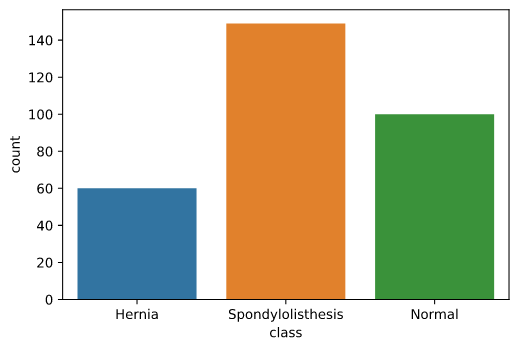
\includegraphics[width=0.425\textwidth]{figures/nbr_individus_par_classe.png}
    \caption{\label{fig:nbr_individus_par_classe}Répartition des individus par classe}
    \end{center}
\end{figure}

\subsubsection{Répartition des variables}

On s'intéresse ensuite à la répartition des variables au sein des différentes classes afin de mettre en évidence les caractéristiques de chaque groupe. On effectue un pivotage du jeu de données du format large au format long sur la composante \textit{class}.

Avec ce jeu de données au format large, on produit des boîtes à moustache (une par classe) des différentes composantes (figure~\ref{fig:boxplot_variables}). Celles-ci nous permettent de comparer la répartition de chaque variable selon les classes d'appartenance.

\begin{figure}[htbp]
    \begin{center}
    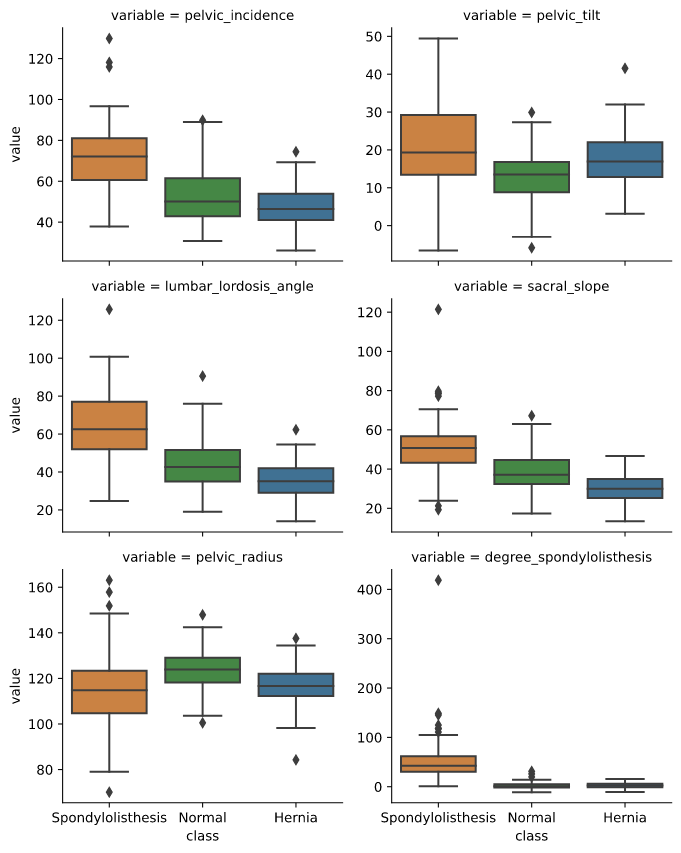
\includegraphics[width=0.425\textwidth]{figures/boxplot_variables.png}
    \caption{\label{fig:boxplot_variables}Répartition des variables}
    \end{center}
\end{figure}

Globalement on remarque pour plusieurs variables une distinction des valeurs de la classe \textit{Spondylolisthesis} (dont la médiane est généralement plus élevée que celle des autres classes sauf pour le \textit{pelvic radius}).
Par contre, les valeurs de \textit{Hernia} et \textit{Normal} sont souvent proches. La répartition des différentes variables ne permet pas de distinguer ces deux classes ce qui justifie notamment une approche multivariée.

\subsubsection{Correction des valeurs aberrantes}
On remarque dans la figure précédente (figure ~\ref{fig:boxplot_variables}) une valeur totalement aberrante au niveau des composantes \textit{degree spondylolisthesis} et \textit{sacral slope}. Il se trouve que c'est le même individu qui possède ces deux valeurs. On choisit donc de le supprimer du jeu de données. On aurait pu lisser le bruit en remplaçant les valeurs aberrantes par la moyenne ou la médiane de la variable correspondante mais puisqu'un seul individu est concerné, cette suppression n'a pas de grandes conséquences sur les résultats. A noter qu'à partir de cette étape, le jeu de données considéré compte 309 individus.

\subsubsection{Répartition des variables 2 par 2}

En comparant les composantes entre elles (2 par 2), il est possible d'effectuer une analyse dimensionnelle complète. On obtient alors une matrice recensant les nuages de points des composantes 2 par 2 (figure~\ref{fig:pairplot}).La diagonale de cette matrice contient les histogrammes de ces composantes.

On distingue 2 clusters: \textit{Hernia-Normal} et \textit{Spondylolisthesis}. Par contre séparer les classes \textit{Normal} et \textit{Hernia} est une tâche plus ardue. On remarque néanmoins quelques différences (et donc une possibilité de clustering) sur certaines composantes, notamment \textit{sacral slope}.

On peut également constater une corrélation entre certaines variables (\textit{pelvic incidence} avec \textit{pelvic tilt}, \textit{lumbar lordosis angle} et \textit{sacral slope}). La variable \textit{pelvic radius} ne semble en revanche corrélée à aucune autre.
\begin{figure}[htbp]
    \begin{center}
    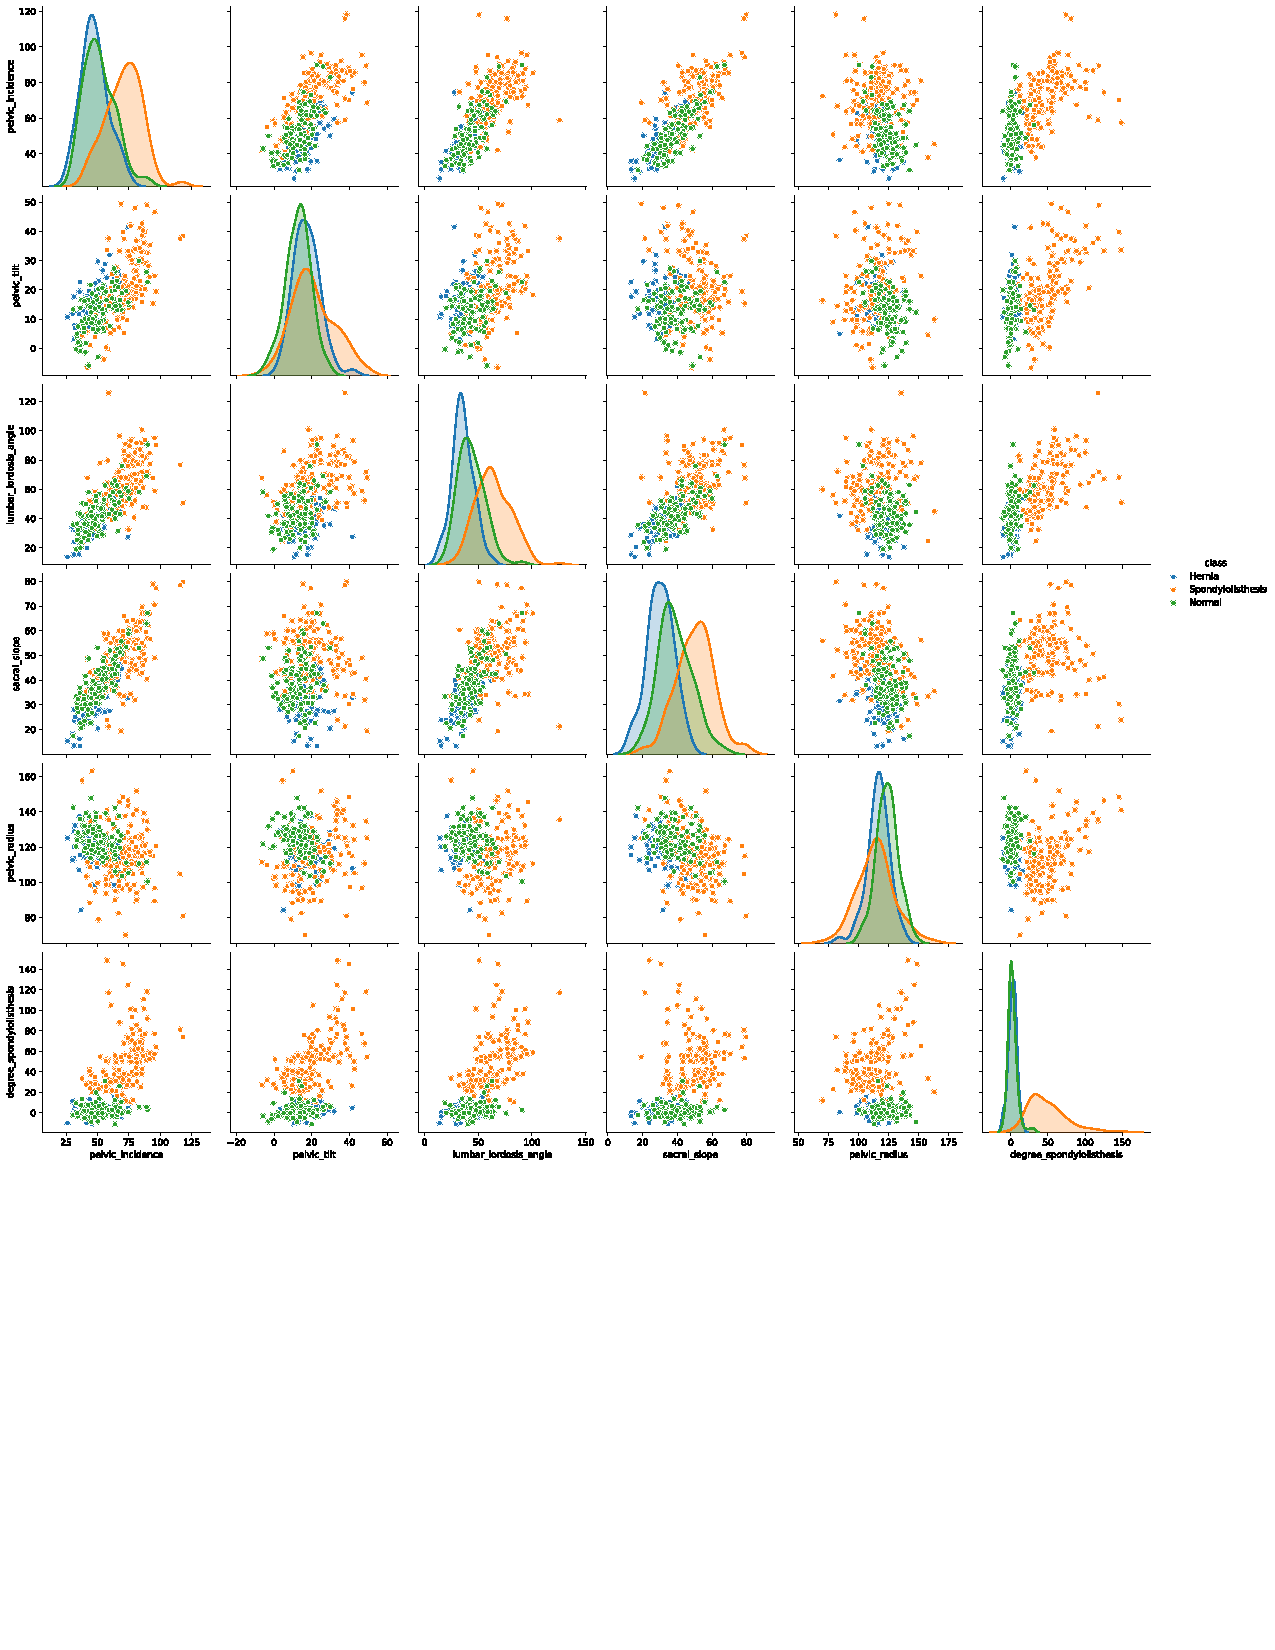
\includegraphics[trim=0 8cm 0 0, width=0.47\textwidth]{figures/pairplot.pdf}
    \caption{\label{fig:pairplot}Répartition des variables 2 par 2 }
    \end{center}
\end{figure}

\subsubsection{Corrélation des variables}
Il s'agit maintenant trouver des relations plus globales sur l'ensemble des composantes. Il est intéressant de faire apparaître une matrice de corrélation entre ces variables(figure~\ref{fig:heat_map_variables}).

On remarque que la composante \textit{pelvic radius} est indépendante des autres composantes (ce qui étaye les observations précédentes). On observe par ailleurs une forte corrélation entre les composantes \textit{sacral slope} et \textit{pelvic incidence}, ainsi qu'entre \textit{pelvic incidence} et \textit{lumbar lordosis angle}.

\begin{figure}[htbp]
    \begin{center}
        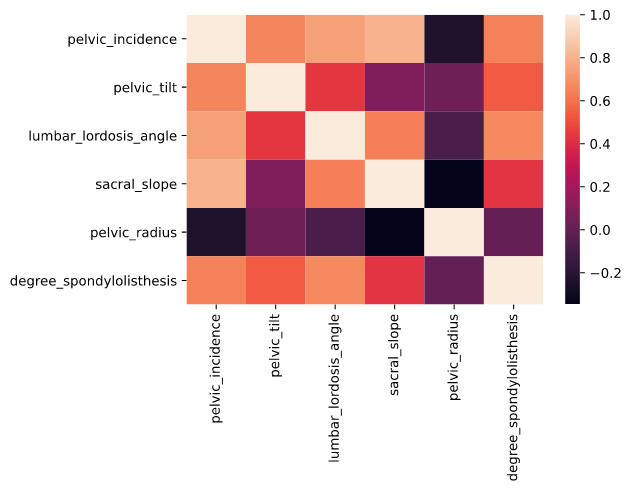
\includegraphics[width=0.425\textwidth]{figures/heat_map_variables.png}
        \caption{\label{fig:heat_map_variables}Corrélation entre les variables}
    \end{center}
\end{figure}

Par définition, on sait que \textit{pelvic incidence} est égal à la somme entre \textit{sacral slope} et \textit{pelvic tilt}. Afin de vérifier cette contrainte dans le cadre de notre étude, nous avons calculé le coefficient de Pearson entre la variable \textit{pelvic incidence} et la variable nouvellement créée \textit{sacral slope + pelvic tilt}. Ce coefficient étant égal à 1, l'hypothèse est validée.

\subsection{Analyse en composantes principales}

Nous avons pu mettre en évidence une corrélation entre plusieurs variables. Il peut être intéressant de diminuer le nombre de variables afin de supprimer les informations redondantes en obtenant des combinaisons linéaires des variables initiales. L'ACP est une méthode adaptée à notre situation puisque l'on dispose d'un tableau individu-variables comportant des valeurs quantitatives.

On applique ainsi l'ACP sur le jeu de données auquel on a retiré l'information de classe. On récupère l'inertie expliquée par les composantes principales obtenues (en pourcentage). A noter qu'on obtiendrait le même résultat avec le fichier \textit{column\_2C\_weka.csv} qui ne diffère que par le nombre de classes étudiées.

Afin de déterminer le nombre d'axes à retenir, on applique la méthode du coude (figure~\ref{fig:inertie_expliquee_ACP}).
On remarque que le 1\ier axe (68.5\%), et le 2\ieme axe (14.6\%) expliquent 81.1\% de l'inertie globale.

\begin{figure}[htbp]
    \begin{center}
        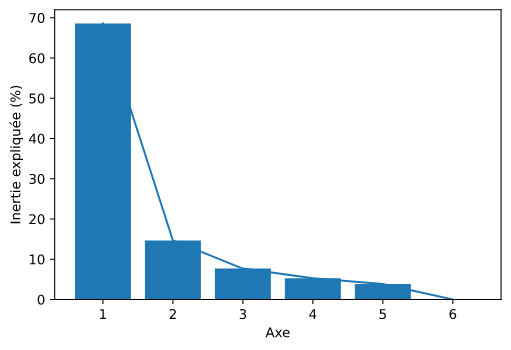
\includegraphics[width=0.425\textwidth]{figures/inertie_expliquee_ACP.png}
        \caption{\label{fig:inertie_expliquee_ACP}Méthode du coude}
    \end{center}
\end{figure}

Sur la figure, on repère visuellement un lieu de rupture après la seconde composante : on choisit donc une représentation dans le premier plan factoriel (figure~\ref{fig:ACP}).

\begin{figure}[htbp]
    \begin{center}
        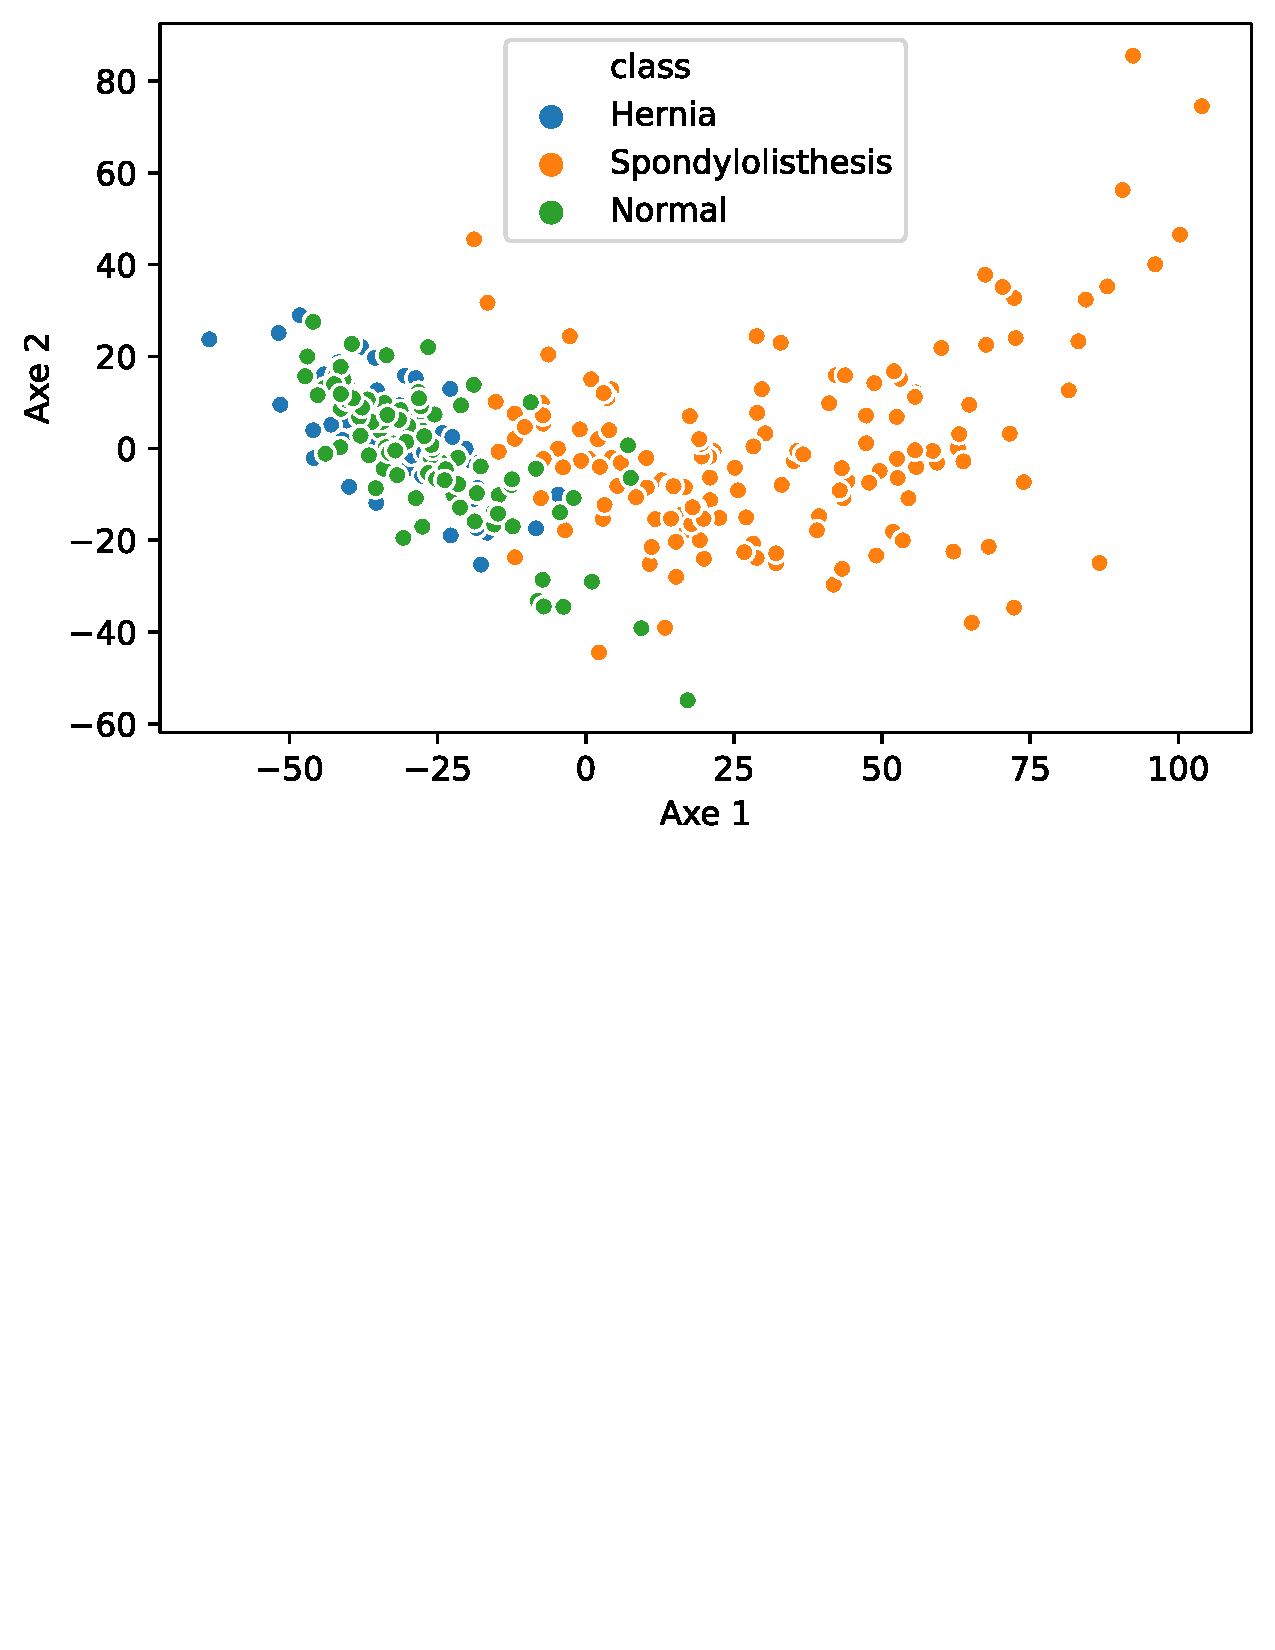
\includegraphics[trim=0 14cm 0 0, width=0.425\textwidth]{figures/ACP.pdf}
        \caption{\label{fig:ACP}Visualisation de l'ACP à 2 composantes}
    \end{center}
\end{figure}

Encore une fois il est possible de distinguer 2 clusters: \textit{Hernia-Normal} et \textit{Spondylolisthesis}. Cela corrobore les observations préalablement réalisées sur le jeu de données, mais ne nous permet pas de séparer clairement les classes \textit{Hernia} et \textit{Normal}.

Le cercle de corrélation (figure~\ref{fig:correlation_circle_ACP}) nous apporte des informations concernant les composantes principales obtenues.

\begin{figure}[htbp]
    \begin{center}
        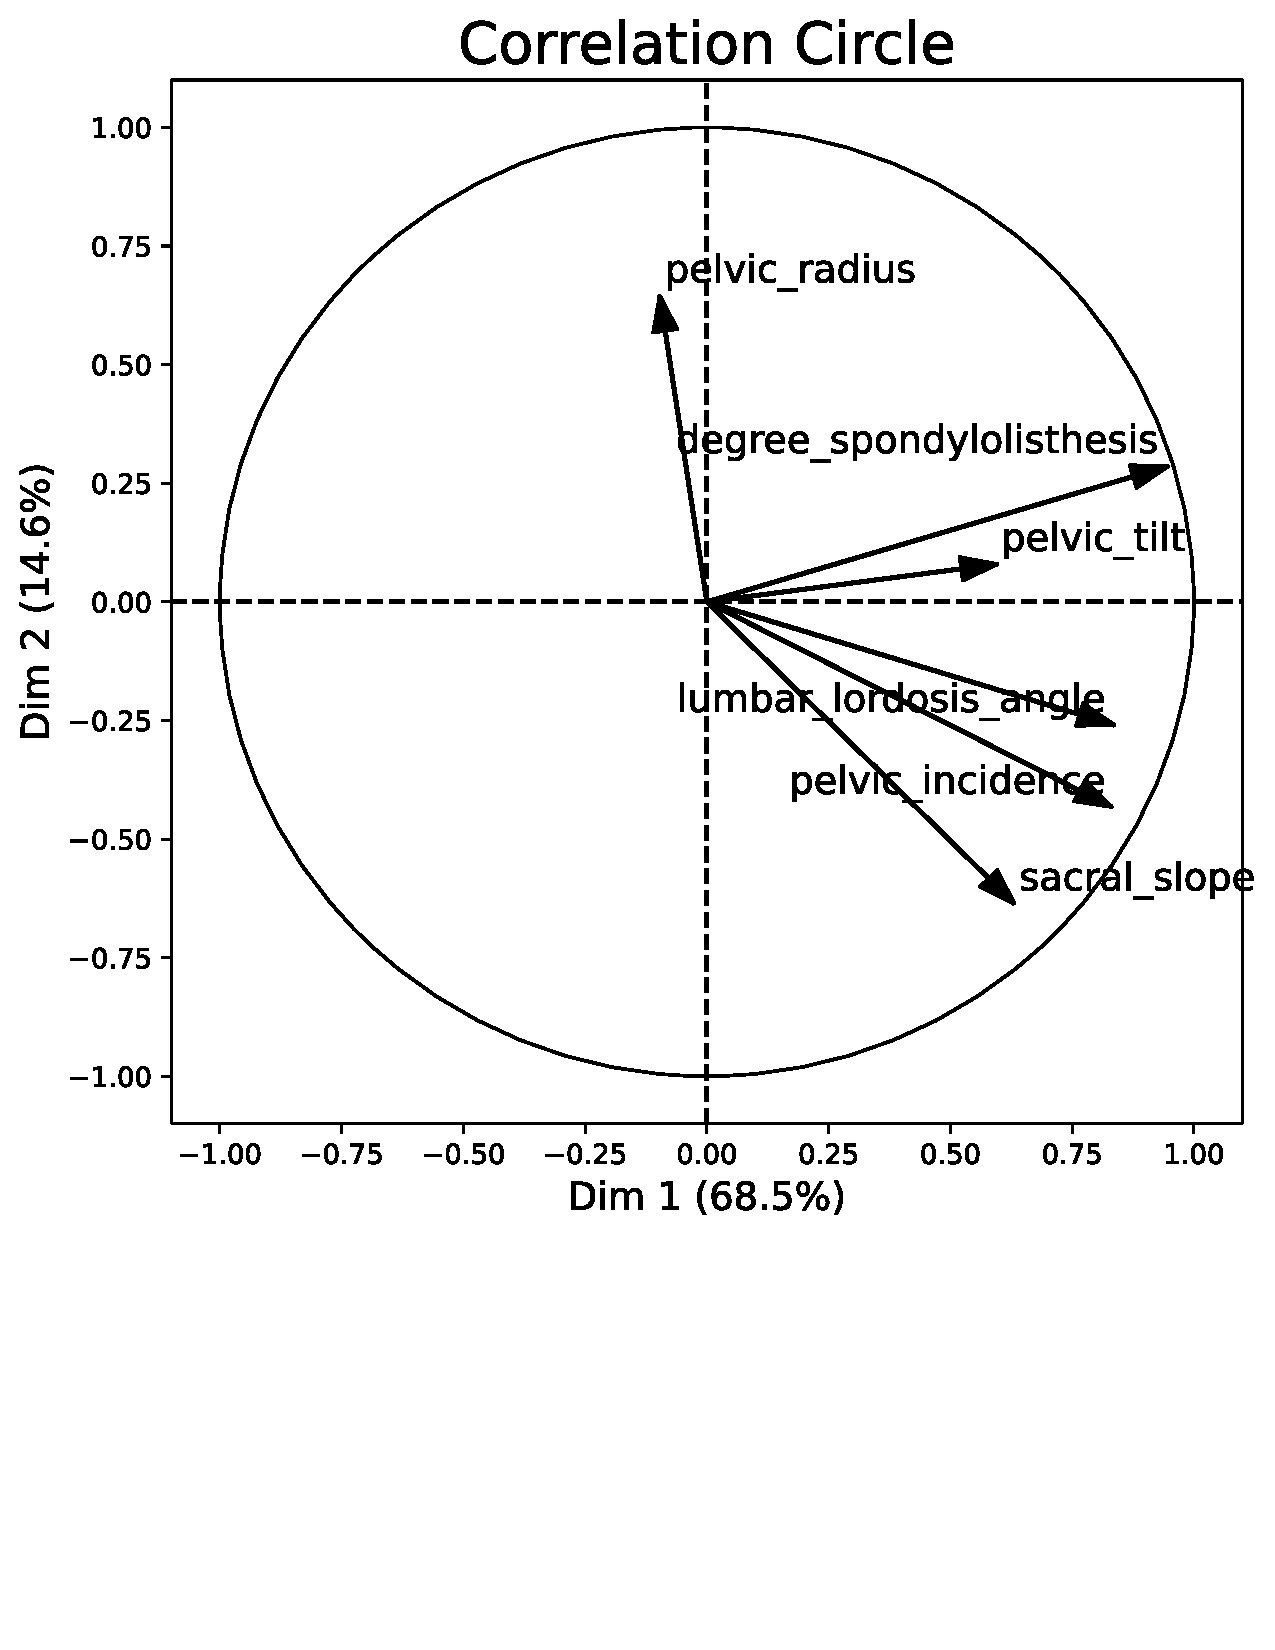
\includegraphics[trim=0 7cm 0 1cm, width=0.4\textwidth]{figures/correlation_circle_ACP.pdf}
        \caption{\label{fig:correlation_circle_ACP}Cercle de corrélation}
    \end{center}
\end{figure}

D'une part, on remarque que la Dimension 2 porte majoritairement l'information du \textit{pelvic radius}. Cela confirme une fois encore l'indépendance de cette variable par rapport aux autres et donc le fait qu'on ne puisse pas l'expliquer par une combinaison des autres descripteurs. La Dimension 1 quant à elle regroupe l'information de l'ensemble des autres variables. On retrouve notamment la corrélation entre les variables \textit{pelvic incidence}, \textit{sacral slope} et \textit{lumbar lordosis angle} relevée précédemment. L'information de cet axe est principalement portée par la variable \textit{degree spondylolisthesis}, associée à la classe de même nom.


\section{Méthodes non-supervisées}

\subsection{Formalisation du problème}

Après exploration des données et mise en évidence de certaines corrélations entre les variables, on constate que dans les différentes représentations du jeu de données, la classe \textit{Spondylolisthesis} se démarque tandis que \textit{Normal} et \textit{Hernia} se confondent. Le but de cette section est de trouver une méthode permettant de prédire de manière efficace l'appartenance d'un individu à l'une de ces classes uniquement à partir des variables descriptives.

On considère donc une population de 309 individus, chacun décrit par 6 caractéristiques qui correspondent à un vecteur forme. La classe correspond quant à elle à la variable à prédire.

\subsection{KMeans}

On applique ainsi la méthode non supervisée des centres-mobiles (ou K-means) qui consiste à affecter chaque individu à la classe dont le centre est le plus proche. Notre connaissance du jeu de données facilite cette recherche de partition car on connaît déjà le nombre réel de classes du jeu de données. On applique donc les K-means pour 3 clusters.

On constate que la partition obtenue est très différente de la partition réelle (alors que le nombre de classes coïncide). En effet, la classe Spondylolisthesis est scindée en deux clusters tandis que les classes Normal et Hernia sont regroupées en une unique classe (figure~\ref{fig:KMeans_3}).
A noter qu'un K-means avec 2 clusters distingue bien la classe \textit{Spondylolisthesis} mais considère les deux autres comme formant un seul et même groupe.

\begin{figure}[htbp]
    \begin{center}
        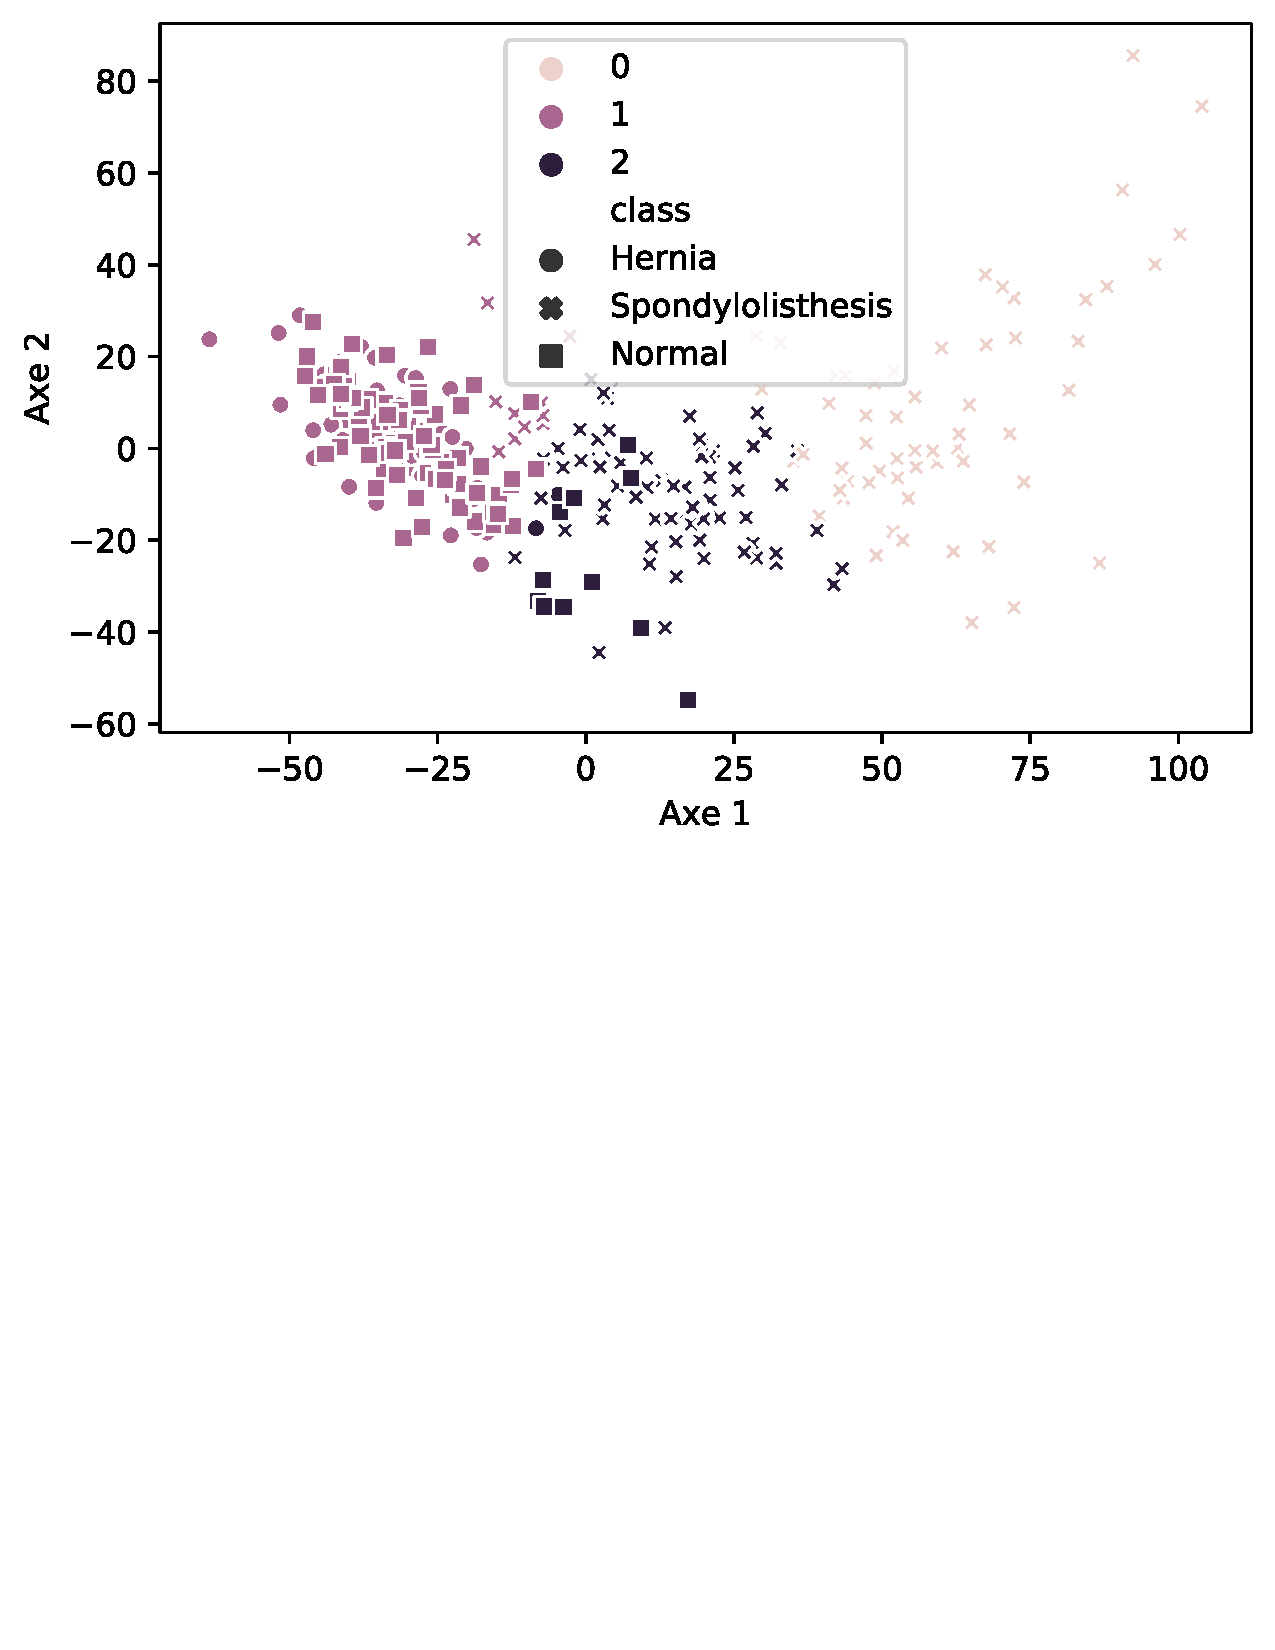
\includegraphics[trim=0 14cm 0 0, width=0.425\textwidth]{figures/KMeans_3.pdf}
        \caption{\label{fig:KMeans_3}Classification d'après la méthode des k-means avec K=3}
    \end{center}
\end{figure}

Le calcul de l'indice de Rand ajusté confirme ces observations puisqu'on obtient, pour K=3, ARI = 0.3085.

On peut donc en conclure que la méthode des K-Means ne nous permet pas de classer correctement les individus des classes Normal et Hernia. L'utilisation de la distance euclidienne ne permet pas ici la création d'une frontière de décision séparant correctement les classes. Étant donné la répartition des clusters, il ne nous semble pas intéressant d'approfondir une démarche non supervisée. Nous faisons donc le choix de ne pas appliquer la méthode des K-means adaptatifs et de nous concentrer d'avantage sur les méthodes supervisées.

\section{Méthodes supervisées}

\subsection{Méthodologie générale}

Ayant constaté des résultats peu concluants avec la méthode de classification des K-Means, le reste de cette étude se focalise sur des méthodes d'analyse supervisées. On sépare ainsi le jeu de données initial en deux sous-ensemble : l'ensemble d'apprentissage et l'ensemble de test (contenant respectivement 2/3 et 1/3 des individus). Il s'agit de faire l'apprentissage des données sur divers modèles puis d'en évaluer les performances.

Compte tenu de la nature des données à notre disposition, nous pourrions définir une fonction de coût qui rendrait plus importantes les conséquences d'une mauvaise classification des individus malades (par exemple classer un individu possédant un hernie dans la classe \textit{Normal}). Toutefois, afin de faciliter la comparaison des performances des différents modèles et puisqu'il s'agit là d'un cas d'étude nous avons décidé de considérer des coûts \{0,1\}. Calculer le risque relatif à chaque classifieur revient donc à calculer les performances de ces mêmes classifieurs.

Enfin, on peut noter que tout au long de cette analyse, le choix d'un meilleur modèle se fonde sur la méthode de validation croisée appliquée sur notre ensemble d'apprentissage initial (à partir duquel on extrait donc un ensemble de validation).


\subsection{KNN}

Dans notre cas les classes ne semblent pas pouvoir être séparées par des frontières linéaires. Une des méthodes applicables est la méthode des K-nearest-neighbors (ou KNN) qui consiste à affecter un individu x à la classe la plus représentée parmi celle de ses K plus proches voisins (au sens de le distance euclidienne).

\subsubsection{Détermination des meilleurs paramètres}

Tout d'abord, il est important de déterminer le nombre de voisins \textit{K} qui optimisera les prédictions (c'est-à-dire tel que le \textit{accuracy score} soit maximisé).
Pour cela on effectue un \textit{GridSearchCV} sur un nombre de voisins variant de 1 à 100. On sélectionne également le meilleur paramètre \textit{weight} du KNN entre \textit{distance} et \textit{uniform}.
Le \textit{GridSearchCv} utilise la validation croisée \textit{StratifiedKFold}, ce qui permet de conserver la répartition d'origine des classes dans chaque Fold. La validation croisée est privilégiée ici par rapport à une validation simple répétée qui engendrerait un risque de sous ou sur-représentation de certains exemples dans l'ensemble d'apprentissage ou de validation.

Il s'agit aussi de déterminer si un pré-traitement sur les données permet d'optimiser le partitionnement obtenu. On peut en effet imaginer appliquer la méthode des KNN sur les données brutes ou transformées (normalisation, ACP, Analyse discriminante linéaire (ADL) Neighborhood Components Analysis(NCA)). Une autre hypothèse consiste en la suppression de la colonne \textit{pelvic\_incidence} qui, étant la somme de \textit{pelvic tilt} et \textit{sacral slope} introduit de la redondance.

Pour chacun de ces ensembles initiaux de données, on applique la méthode des KNN puis on retourne le meilleur score de validation obtenu (via le \textit{GridSearchCv}) et la valeur k associée à ce score (présentés dans le tableau \ref{tab:accuracy_KNN}).

\begin{table}[htbp]
    \begin{center}
        \caption{\label{tab:accuracy_KNN}Meilleur score de validation par méthode de pré-traitement}
        \begin{tabular}{c|ccc}
            \multirow{2}{*}{Méthode} & Meilleur & \multirow{2}{*}{K} & \multirow{2}{*}{weights} \\
            & score & \\
            \hline
            Données brutes & 85.42 \% & 5 & distance \\
            MinMaxScaler & 81.98 \% &  9 & distance\\
            StandardScaler & 81.53 \% &  17 & distance\\
            ACP (2) & 79.59 \% & 4 & distance \\
            NCA & 86.85 \% & 1 & uniform\\
            NCA (2) & 89.76 \% & 6 & distance\\
            ADL & 86.85 \% & 1 & uniform\\
            ADL (2) & 89.76 \% & 6 & distance\\
            Sans pelvic incidence & 86.87 \% & 9 & distance \\ \hline
            Sans pelvic incidence  &  \multirow{2}{*}{89.77 \%} & \multirow{2}{*}{1} & \multirow{2}{*}{uniform}\\
            + NCA (2) & & \\ 
            \textit{StandardScaler}  &  \multirow{2}{*}{\textit{90.74 \%}} & \multirow{2}{*}{\textit{14}} & \multirow{2}{*}{\textit{distance}}\\
            \textit{+ NCA (2)} & & \\
            StandardScaler  &  \multirow{2}{*}{87.34 \%} & \multirow{2}{*}{48} & \multirow{2}{*}{uniform}\\
            + ADL (2) & & \\ 
            MinMaxScaler  &  \multirow{2}{*}{90.26 \%} & \multirow{2}{*}{85} & \multirow{2}{*}{distance}\\
            + NCA (2) & & \\ 
            MinMaxScaler  &  \multirow{2}{*}{87.34 \%} & \multirow{2}{*}{48} & \multirow{2}{*}{uniform}\\
            + ADL (2) & & \\ 

        \end{tabular}
    \end{center}
\end{table}

D'autres combinaisons de paramètres ont également été testées mais nous avons décidé de ne conserver que les pré-traitements intéressants dans le cadre de notre étude.

On peut voir que c'est en utilisant les données transformées avec un \textit{Neighborhood Components Analysis} à deux composantes associée à un \textit{Standard Scaler} et avec \textit{distance} comme \textit{weights} que l'on obtient la meilleure \textit{accuracy} (90.74\%), pour \textit{k=14} (figure~\ref{fig:KNN_cross_val}).

\begin{figure}[htbp]
    \begin{center}
        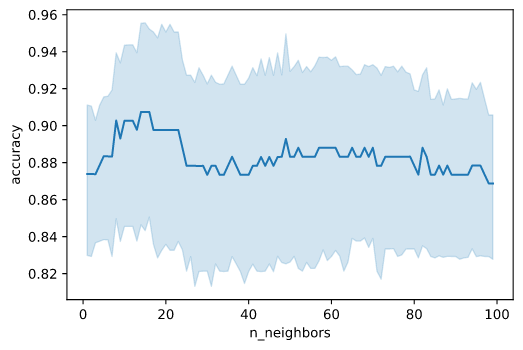
\includegraphics[width=0.425\textwidth]{figures/KNN_cross_val.png}
        \caption{\label{fig:KNN_cross_val}Résultat de la validation avec différents nombres de voisins}
    \end{center}
\end{figure}

\subsubsection{Analyse des résultats}

La plupart des algorithmes de Machine Learning nécessitent une mise à l'échelle des données visant à améliorer les performances et les résultats obtenus. Dans le cas du KNN, une normalisation des données est censée améliorer les résultats. En effet, cette méthode se base sur une mesure de la distance, ce qui peut aboutir à de mauvaises performances si on dispose de variables avec des unités et des ordres de grandeur différents.
Nous avons donc choisi d'appliquer les techniques de MinMaxScaler et StandardScaler fournies par Scikit-Learn. La première consiste à transformer les caractéristiques en les adaptant à une plage donnée (ici [0, 1]). La deuxième transforme les données par centrage et réduction. On constate néanmoins que les résultats obtenus après normalisation sont moins bons que ceux obtenus à partir des données brutes.
Dans notre cas la plupart des variables sont des angles, leurs unités et ordres de grandeur sont donc semblables ce qui peut rendre une telle normalisation inutile. Néanmoins, cela n'explique pas l'obtention de moins bons résultats.

En revanche, il n'est pas surprenant de voir des résultats assez faibles pour l'ACP, puisque les axes pris n'expliquent pas toute la répartition des données. Il serait intéressant d'utiliser l'ACP, et donc de sacrifier un peu de précision, si on avait un nombre de variables initiales important, et que l'algorithme prenait trop de temps à s'exécuter.
Or dans notre cas il y a seulement 6 variables et le KNN est rapide. On abandonne donc ce jeu de données dans le cadre de cette méthode.

En plus de l'ACP, nous avons identifié deux autres méthodes de pré-traitement: l'Analyse discriminante linéaire (ADL) et la Neighborhood Components Analysis(NCA) \cite{scikit-learn-Dimensionality-Reduction}. Contrairement à l'ACP, ces deux méthodes sont des méthodes de pré-traitement supervisées. La NCA permet d'apprendre une métrique de distance qui améliore les performances du KNN par rapport à la distance euclidienne classique. L'algorithme maximise le score d'un \textit{Leave-one-out-knn}, (où $K=N-1$ avec $N$ le nombre de points). Il permet ainsi de transformer les données et de réduire le nombre de dimensions \cite{scikit-learn-neighborhood-components-analysis}. L'ADL quant à elle permet de réduire le nombre de dimensions en maximisant la séparation des classes (en se basant sur la variance entres celles-ci). On remarque que la NCA et l'ADL sont plus performantes avec une réduction de dimension. On peut voir également que la NCA combinée au KNN est plus performante que l'ADL, dans le cas où on applique une normalisation des données préalablement. 

Par ailleurs, notre intuition sur la redondance des données causée par \textit{pelvic\_incidence} s'avère être correcte puisqu'on obtient de meilleurs résultats en enlevant cette variable du jeu de données.

Nous avons enfin vérifié l'impact du paramètre weights du KNN. Par défaut, il prend la valeur \textit{uniform}. Mais avec la valeur \textit{distance}, le KNN donne un poids plus important aux points les plus proches. Dans certains cas la modification de cette valeur par défaut permet d'améliorer les performances.

\subsubsection{Analyse du meilleur KNN}

En appliquant le meilleur modèle à l'ensemble de test on obtient un score de test de 81.55 \%. La frontière de décision pour le meilleur KNN est représentée dans la figure \ref{fig:decision_boundary}.

\begin{figure}[htbp]
    \begin{center}
        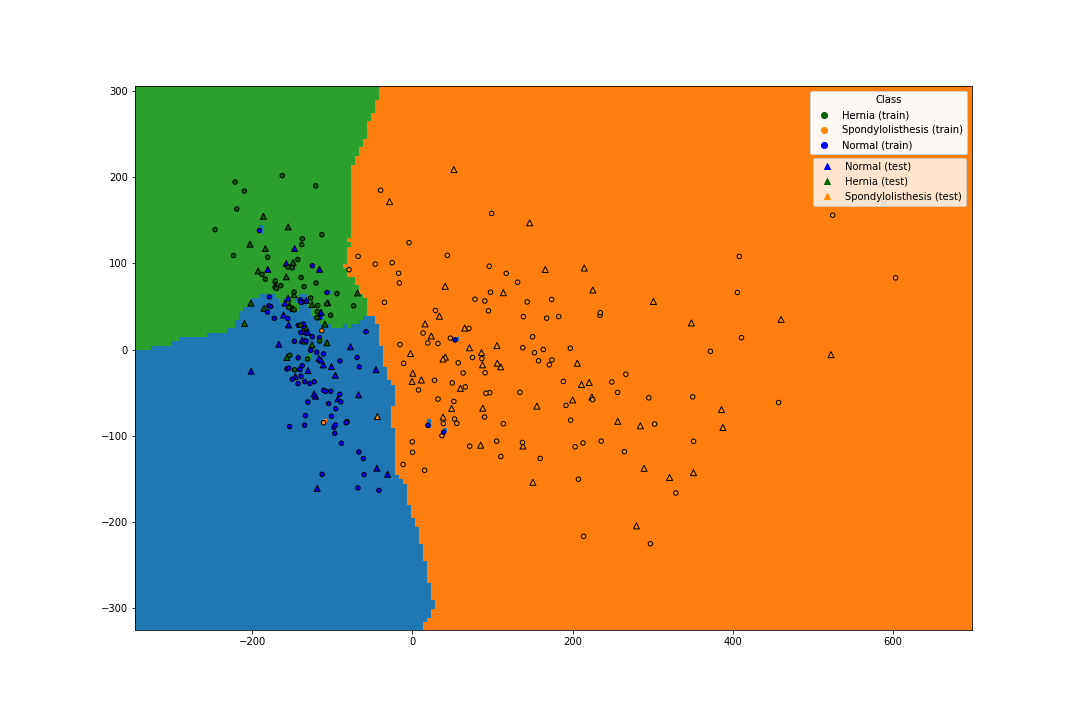
\includegraphics[width=0.5\textwidth]{figures/decision_boundary_knn.png}
        \caption{\label{fig:decision_boundary}Frontière de décision pour le KNN}
    \end{center}
\end{figure}

On remarque tout d'abord que la NCA permet de mieux séparer les classes, par rapport à l'ACP (figure ~\ref{fig:ACP}) ce qui justifie notamment les meilleurs résultats obtenus suite à ce pré-traitement. On peut également distinguer ce qui semble être un léger \textit{overfitting}. On peut par exemple voir une région (de taille infime) qui est considérée comme \textit{Normal} à cause d'un seul point dans la région \textit{Hernia}.
Cela peut être expliqué par le fait que le paramètre \textit{K} n'est pas très élevé (5), mais surtout parce qu'on utilise \textit{distance} pour le paramètre \textit{weights}. Ainsi, si un point est excentré par rapport aux autres, il aura plus de poids dans la classification de la région autour de lui. Ce qui est bien le cas dans notre exemple.

Par ailleurs, on a représenté les points de l'ensemble de test (points en forme de triangle). Ils correspondent aux vraies classes des individus de test. Les afficher nous permet notamment de comprendre la différence constatée entre la test et la validation accuracy.
On peut ainsi voir plusieurs points de \textit{Hernia} de l'ensemble de test qui sont mélangés aux points de \textit{Normal} et inversement. Ces points n'ont donc pas été pris en compte lors de l'apprentissage et ne sont donc pas du "bon coté" de la frontière de décision. Cette hypothèse est confirmée si on modifie la division entre les ensembles d'entraînement et de test, puisqu'on obtient une test accuracy différente en fonction du split initial.


\subsection{Analyse discriminante}

Nous avons vu dans la section précédente que la méthode des KNN permettait globalement de classer les individus mais avait des difficultés à distinguer les classes \textit{Hernia} et \textit{Normal}. Nous avons également mis en évidence l'efficacité de certaines méthodes de pré-traitement tels que la NCA et la LDA. Outre sa fonction de pré-traitement, il est important de noter que l'analyse discriminante linéaire est également une méthode d'apprentissage à part entière, particulièrement populaire dans le domaine de la biologie. Au sein de cette section, nous détaillerons 3 modèles d'analyse discriminante : l'analyse discriminante linéaire, quadratique et le classifieur bayésien naïf, chacun consistant en une expression particulière de la règle de Bayes.

\subsubsection{Hypothèse de normalité}

Il faut savoir que ces méthodes s'appliquent généralement sous l'hypothèse que chaque classe suive une loi normale multidimensionnelle. Toutefois il est possible de les utiliser lorsque ce n'est pas le cas \cite{Aide-mémoiredestatistiqueappliquéeàlabiologie}.

On cherche à tester cette hypothèse grâce au test de Shapiro-Wilk. On considère un niveau de signification $\alpha$* égal à 0.05.
On obtient des \textit{p-values} très faibles (respectivement 1.5846e-21, 2.6126e-18 et 2.2085e-11) et donc inférieures à $\alpha$*. On rejette donc l'hypothèse par défaut de normalité conditionnellement à la classe. On peut conclure avec un niveau de confiance de 95\% que les données ne suivent pas une loi normale.

En second recours et afin d'améliorer ces résultats, on cherche à normaliser les données avec un pré-traitement de standardisation, par exemple \textit{StandardScaler} (centrage et réduction). On renouvelant le test de Shapiro sur les données standardisées, on obtient des \textit{p-values} plus élevées. Cependant, dans le cas des \textit{Normal} et \textit{Spondylolisthesis}, elle reste inférieure à 0.05 ce qui nous amène une fois encore à rejeter l'hypothèse nulle. A l'inverse pour \textit{Hernia} on obtient \textit{p-value = 0.123} : on ne peut pas rejeter l'hypothèse de normalité.

Le tableau suivant répertorie les \textit{p-values} pour chaque classe avant et après l'application du standardiseur.
\begin{table}[htbp]
    \begin{center}
        \caption{\label{tab:p_value_shapiro}p-values calculées par le test de Shapiro}
        \begin{tabular}{c|cc}
          Classe & Sans pré-traitement & StandardScaler \\
            \hline
            Normal & 1.58e-21 & 4.11e-9 \\ 
            Hernia & 2.61e-18 & 0.12 \\
            Spondylolithesis & 2.21e-11 & 3.06e-7 \\ 
        \end{tabular}
    \end{center}
\end{table}

On déduit de ces résultats que les données ne valident pas l'hypothèse émise initialement (mise à part pour la classe \textit{Hernia} après pré-traitement). Comme mentionné précédemment, cela n'interdit pas le recours à cette méthode celle-ci étant robuste et pouvant supporter des données non-normalisées.Toutefois on pourra s'attendre à des résultats moins satisfaisants, 

\subsubsection{Pré-traitements}
Il s'agit ici de déterminer les pré-traitements à appliquer aux données d'apprentissage pour obtenir des résultats optimaux. La standardisation appliquée au jeu de données à permis de centrer-réduire les variables. Le test de Shapiro a également mis en évidence la normalité de la classe \textit{Hernia} suite à une telle transformation. On pourrait alors penser qu'appliquer un \textit{Scaler} comme pré-traitement pour une analyse discriminante permettrait d'obtenir des résultats plus satisfaisants. Cependant, la standardisation d'un ensemble de données ne modifie pas les valeurs propres de la matrice associée. La discrimination inter-classe qui se base sur ces valeurs propres reste alors inchangée \cite{Standardizing_features_when_using_LDA_as_a_pre-processing_step}. Cela pourrait donc expliquer les résultats du Standard Scaler qu'on obtient dans le tableau \ref{tab:accuracy_analyse_discriminante}
%Il en va de même pour l'analyse de voisinage. 


Un autre élément à prendre en compte est la sensibilité de l'analyse discriminante à la colinéarité. Il faut en effet retirer la composante
\textit{pelvic-incidence} (qui, comme mentionné précédemment, est source de redondance) pour optimiser les résultats du modèle. Ce pré-traitement est d'autant plus nécessaire que le classifieur bayésien naïf a pour hypothèse l'indépendance des variables conditionnellement à chacune des classes. En retirant la variable \textit{pelvic-incidence}, on augmente les chances d'obtenir des résultats satisfaisants pour ce classifieur.

Par ailleurs, l'analyse quadratique étant sensible au nombre de composantes, on peut tenter de les faire varier grâce à une ACP sur les données. Les résultats de cette variation sont synthétisés dans le tableau \ref{tab:accuracy_analyse_discriminante}.

\begin{table}[htbp]
    \begin{center}
        \caption{\label{tab:accuracy_analyse_discriminante}Score de validation de l'analyse discriminante par méthode de pré-traitement}
        \begin{tabular}{c|ccc}
          Modèles & Linaire & Quadratique & Gaussien \\
            \hline
            Brute & 83.88 \% & \textit{84.48 \%} & 83.90 \% \\
            ACP 4 & 83.38 \% & 84.35 \% & 83.38 \% \\
            ACP 3 & 80.90 \% & 83.88 \% & 80.00 \% \\
            ACP 2 & 72.30 \% & 70.38 \% & 69.45 \% \\
            ACP 1 & 72.21 \% & 72.21 \% & 70.29 \% \\
            Standard Scaler & 83.88 \% & 84.48 \% & 83.90 \% \\
            NCA & 83.88 \% & 84.48 \% & 83.90 \% \\
        \end{tabular}
    \end{center}
\end{table}

\subsubsection{Résultats}

Au terme de ces diverses expérimentations, on remarque que l'on obtient de manière générale de meilleurs résultats à partir des données brutes, ce qui est intuitivement logique puisque l'ACP est susceptible de causer des pertes d'informations. C'est en particulier à partir des données brutes et en utilisant le modèle d'analyse discriminante quadratique qu'on obtient le meilleur score de validation croisée sur l'ensemble d'apprentissage. Nous avons évoqué précédemment le fait que l'analyse discriminante quadratique était sensible à la dimension de l'espace. En effet, plus le nombre de variables augmente, plus le nombre de paramètres à estimer croît. Dans notre cas, et malgré le peu d'individus d'apprentissage dont nous disposons, le nombre de variable est suffisamment faible pour limiter les erreurs d'estimation. De plus parmi les 3 méthodes considérées, c'est celle qui est la plus flexible en termes d'hypothèses ce qui explique les bons résultats obtenus.

A partir de ce modèle optimal, on prédit les labels de l'ensemble de test que l'on compare aux classes réelles : on obtient un score de test égal à 79.61.

\subsection {Régression logistique}

Nous avons vu dans la méthode précédente que sous certaines hypothèses sur les données, il était possible d'exprimer la règle de Bayes et ainsi de prédire l'appartenance aux classes. En revanche, ces estimations peuvent s'avérées imprécises lorsque les hypothèses ne sont pas vérifiées. Une alternative est la régression logistique, fréquemment utilisée pour la détection de maladies. Dans notre cas il s'agit d'appliquer une régression logistique multinomiale (en raison des 3 classes à prédire) sur notre jeu de données.

\subsubsection{Sélection des pré-traitements}
Comme pour les méthodes précédentes, il s'agit de sélectionner le pré-traitement à appliquer sur l'ensemble d'apprentissage pour optimiser les performances du modèle. On peut par exemple étudier la méthode de pré-traitement supervisée du Neighborhood Components Analysis détaillée dans la section relative au KNN. Une autre méthode de réduction envisagée est l'ACP.

On s'interroge aussi sur l'influence d'une standardisation des données via les fonction MinMaxScaler ou StandardScaler. Enfin une des conditions d'application de cette méthode est la non-colinéarité des variables. On calcule donc le score d'apprentissage après avoir supprimé la colonne \textit{pelvic incidence}. Ces différents pré-traitements sont appris successivement par le module de régression logistique qui utilise les paramètres par défaut.

\begin{table}[htbp]
    \begin{center}
        \caption{\label{tab:accuracy_LogReg}Meilleur score de validation par méthode de pré-traitement}
        \begin{tabular}{c|cc}
            {pré-traitement} & Score de validation \\
            \hline 
            Aucun & 83.47 \%  \\
            Sans pelvic incidence & 85.40 \% \\
            StandardScaler & 83.47 \% \\
            MinMaxScaler & 82.52 \% \\
		    NCA (2) & 84.42 \% \\
			ACP (2) & 73.73 \% \\
			\textit{Sans pelvic incidence} & \multirow{2}{*}{\textit{85.90 \%}}  \\
            \textit{+ NCA (2)} & \\
        \end{tabular}
    \end{center}
\end{table}

Le tableau \ref{tab:accuracy_LogReg} montre que la standardisation et la mise à l'échelle des données est inutile dans le cadre de cette méthode. Par ailleurs, le score d'apprentissage sur les données obtenues par ACP est nettement inférieur à celui obtenu à partir des données brutes (probablement car l'ACP n'explique pas toutes les informations portées par les données initiales). On rejette donc ce pré-traitement. En revanche, et comme les hypothèses laissaient présager, la suppression de la variable \textit{pelvic incidence} améliore les résultats. De même, on constate des résultats intéressants suite à une \textit{Neighborhood Components Analysis}. On constate ainsi que parmi toutes les combinaisons de pré-traitement des données, le meilleur score d'apprentissage (85.90\%) est obtenu à partir des données auxquelles on a appliqué successivement une suppression de la colonne \textit{pelvic incidence} et une NCA à 2 composantes.

\subsubsection{Choix des paramètres de régression}

Un des paramètres du modèle intéressant dans le cadre d'une régression logistique est le "`solver"'. Il en existe 5 :
\begin{itemize}
	\item \textit{newton-cg}: la méthode de Newton calcule la matrice héssienne exacte. Cette exactitude dans les calculs peut néanmoins entraîner des coûts importants pour les jeux de données de taille conséquente (ce qui n'est pas notre cas).
    \item \textit{lbfgs} : cette méthode, similaire à la précédente consiste à approximer les dérivées secondes. Il s'agit de la méthode par défaut et donne des résultats satisfaisant dans la plupart des cas.
    \item \textit{liblinear}: l'algorithme minimise une fonction multivariée en résolvant de manière itérative des problèmes d'optimisation univariés. En revanche cette méthode ne peut pas apprendre de modèle multinomial, se contentant de décomposer le problème en "`une classe VS le reste"'. Nous décidons donc d'ignorer ce solver.
    \item \textit{sag} (Stochastic Average Gradient descent): c'est une variation de l'algorithme du gradient qui utilise un échantillon aléatoire de gradients précédemment calculés.
    \item \textit{saga} : ce solver est une extension de la méthode sag.

\end{itemize}

A l'aide du module GridSearchCV (qui effectue une validation croisée sur 5 plis), on teste les différents solver énumérés ci-dessus sur le pré-traitement optimal introduit précédemment.

\begin{table}[htbp]
    \begin{center}
        \caption{\label{tab:accuracy_LogReg_solver}Meilleur score de validation par solver}
        \begin{tabular}{c|cc}
            {Solver} & Score de validation \\
            \hline
            newton-cg & 85.90 \%\\
            lbfgs & 85.90 \%\\
            sag & 76.19 \% \\
            saga & 76.19 \% \\
        \end{tabular}
    \end{center}
\end{table}

\subsubsection{Analyse des résultats}

Les meilleurs résultats sont obtenus avec les méthodes \textit{lbfgs} et \textit{newton-cg}. Cela n'est pas surprenant pour le solver \textit{newton-cg} qui calcule la matrice hessienne exacte. La méthode \textit{lbfgs} est également souvent utilisée car efficace et économe en mémoire, surtout pour les jeux de données de taille faible. De plus ces deux méthodes sont robustes dans le cas de données sans mise à l'échelle ce qui explique les bons résultats obtenus. En revanche, les méthodes \textit{sag} et \textit{saga} produisent généralement des meilleurs résultats sur des données centrées-réduites ce qui peut justifier leur faible score.

Ainsi, en utilisant le solver \textit{newton-cg} pour une régression logistique appliquée aux données de test pré-traitées, on obtient un score de test de 84.47\%. 

Il est également intéressant d'analyser le score par classe, puisqu'on pouvait voir avec l'ACP (figure~\ref{fig:ACP}) qu'il n'y avait qu'une seule classe qui était bien séparée des autres. On calcule pour cela la matrice de confusion (figure~\ref{fig:confusion_matrix_LR}) relative au meilleur modèle appliqué à l'ensemble de test.
On peut voir que la classe \textit{Spondylolisthesis} est très bien prédite (98\%), contrairement à \textit{Hernia} (55\%) qui est souvent (45\%) confondue avec \textit{Normal} (82\%).

\begin{figure}[htbp]
    \begin{center}
        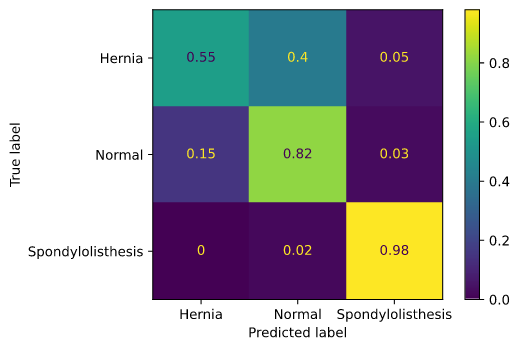
\includegraphics[width=0.425\textwidth]{figures/confusion_matrix_Logistic_Regression.png}
        \caption{\label{fig:confusion_matrix_LR}Matrice de confusion pour la Régression Logistique}
    \end{center}
\end{figure}

La frontière de décision résultant de cet apprentissage est représentée dans la figure \ref{fig:decision_boundary_LR}

\begin{figure}[htbp]
    \begin{center}
        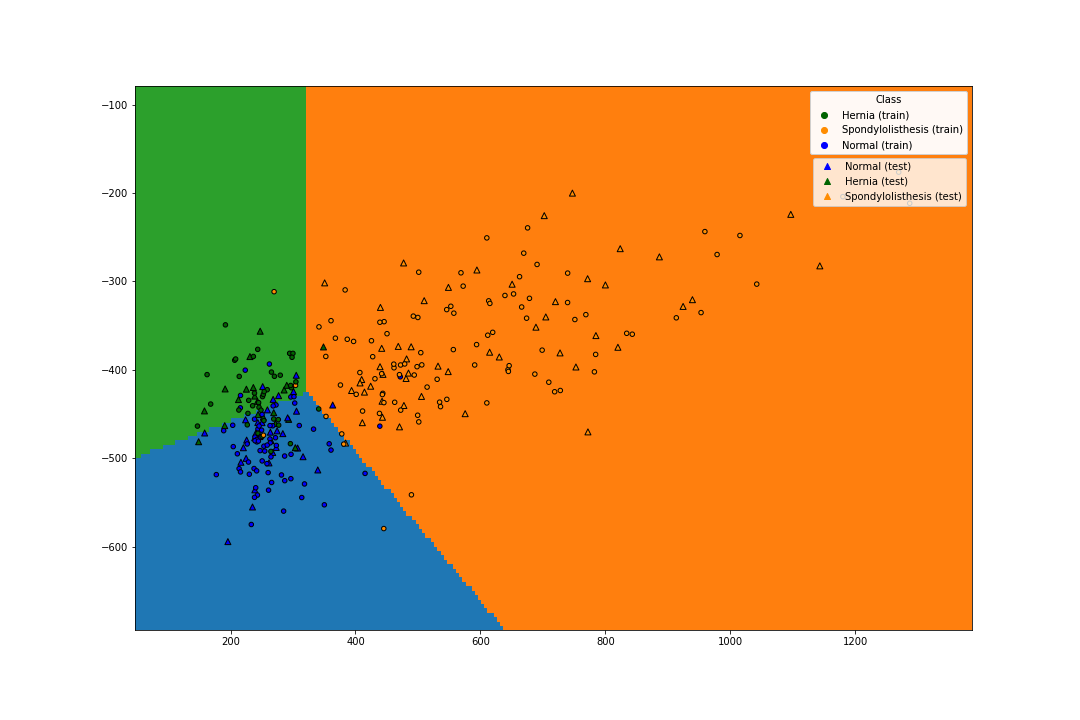
\includegraphics[width=0.5\textwidth]{figures/Decision_boundary_Logistic_Regression.png}
        \caption{\label{fig:decision_boundary_LR}Frontière de décision pour la régression logistique}
    \end{center}
\end{figure}


\subsubsection{Interprétation des coefficients}

Il est par ailleurs intéressant d'analyser les coefficients obtenus suite à l'apprentissage d'un modèle afin de mettre en évidence la prépondérance de certaines variables dans la décision de classification. Or, étudier ces coefficients sur les données pré-traitées n'a que peu d'intérêt puisque les axes considérés ne sont pas explicites aux vues de notre cas d'étude. Nous décidons ainsi de retenir le second meilleur modèle en terme de score de validation, que l'on a obtenu à partir des données auxquelles on a simplement retiré la variable \textit{pelvic incidence}.

Grâce à la classe MNLogit du module \textit{statsmodels}, on estime donc les coefficients de régression logistique multinomiale. On choisit comme groupe de référence la classe \textit{Normal}. Cela signifie que les coefficients obtenus représentent les logit des variations des variables prédictives considérées par rapport aux valeurs de la classe de référence, en supposant les autres variables constantes. Ces coefficients sont obtenus par maximum de vraisemblance.

On applique le test de Wald pour tester la significativité des coefficients. Dans un soucis de simplification des résultats observés, nous avons décidé de ne représenter dans un tableau que les résultats obtenus pour la classe \textit{Hernia} qui se rapproche d'avantage de la classe de référence que \textit{Spondylolisthesis}. On regroupe ainsi les coefficients $\beta$, le z-score et la p-value associée à cette statistique dans le tableau \ref{tab:interpretations_coef_Hernia}.

\begin{table}[htbp]
    \begin{center}
        \caption{\label{tab:interpretations_coef_Hernia} Estimation des coefficients de Régression Logistique pour la classe Hernia}
        \begin{tabular}{c|ccc}
            Variables & Coef. & Z & P>|z| \\
            \hline
            const & 21.2171 & 3.958 & 0.000 \\
            pelvic\_tilt & 0.0789 & 1.619	 & 0.105\\
            lumbar\_lordosis\_angle & -0.0291 & -0.658 & 0.510\\
            sacral\_slope & -0.1915 & -3.527	& 0.000 \\
            pelvic\_radius & -0.1270 & -3.554 & 0.000	\\
			degree\_spondylolisthesis & 0.0283 & 0.580	& 0.562\\

        \end{tabular}
    \end{center}
\end{table}

La probabilité que la statistique de test soit aussi extrême que la valeur obtenue ici est définie par P>|z|. En considérant un niveau de signification égal à 0.05, les p-values des statistiques de test z pour les descripteurs \textit{sacral\_slope} et \textit{pelvic\_radius} sont suffisamment faibles pour rejeter l'hypothèse nulle. On peut donc conclure que les coefficients relatifs à ces variables sont statistiquement différents de zéro et sont donc significatifs pour la classe \textit{Hernia} comparée à la classe \textit{Normal}. On peut donc s'appuyer sur ces variables afin de mieux distinguer les classes Hernia et Normal.

A titre indicatif, pour la classe \textit{Spondylolisthesis}, le coefficient associé à la variable \textit{degree\_spondylolisthesis} est égal à 0.2803 ce qui renvoie z=5.032 et donc une probabilité P>|z| égale à 0.000. Le coefficient de cette variable est donc significatif. Cela conforte nos hypothèses sur l'importance de cette variable dans la classification des individus du groupe \textit{Spondylolisthesis}.


\subsection{Forêt aléatoire}

Enfin, nous décidons d'approfondir notre analyse du jeu de données en appliquant la méthode dite de la forêt aléatoire (Random Forest), très populaire en apprentissage supervisé.

\subsubsection{Choix des pré-traitements et des paramètres }
Nous commençons encore une fois par déterminer le meilleur pré-traitement à appliquer à nos données.
Nous avons pour cela exploré plusieurs méthodes: enlever \textit{pelvic\_incidence}, transformer les données avec un StandardScaler, un MinMaxScaler mais aussi avec un NCA.
Le NCA est classiquement utilisé avec un KNN. Cependant, aux vues de ses bons résultats pour séparer les classes (figure~\ref{fig:decision_boundary}), nous tentons tout de même de l'appliquer à la méthode de la forêt aléatoire.

La deuxième étape est la détermination des meilleurs paramètres. Nous nous sommes intéressés aux avons paramètres suivants:
\begin{itemize}
    \item \textit{criterion} : le critère utilisé pour évaluer la qualité d’une séparation (\textit{gini}, \textit{entropy}).
    \item \textit{max\_features} : le nombre de caractéristiques à retenir de manière aléatoire pour la recherche de la meilleure séparation (2, 3, 4, 5, None(toutes les caractéristiques)).
    \item \textit{n\_estimators} : le nombre d’arbres utilisés dans la forêt (10, 100, 200, 300).
    \item \textit{bootstrap}: la réalisation de l’entraînement sur toutes les données ou sur un échantillon aléatoire (True, False)
    % \item \textit{max\_leaf\_nodes} : le nombre maximum de feuilles autorisée lors de la construction de l’arbre.
    % \item \textit{max\_depth} : la profondeur maximale autorisée lors de la construction de l’arbre.
    % \item \textit{ccp\_alpha} : paramètre $\lambda$ utilisé pour l’élagage coûtcomplexité.
\end{itemize}

Afin de tester ces paramètres nous effectuons un \textit{GridSearchCV}, sur toutes les méthodes de pré-traitement à chaque fois.

\subsubsection{Résultats}

Le tableau \ref{tab:accuracy_RF} indique les meilleurs résultats obtenus pour chacune des méthodes détaillées précédemment. 
\begin{table}[htbp]
    \begin{center}
        \caption{\label{tab:accuracy_RF}Meilleur score de validation par méthode de pré-traitement}
        \begin{tabular}{c|cc}
            \multirow{2}{*}{Méthode} & \multirow{2}{*}{Données brutes} & Sans pelvic \\
                                     &                                 & incidence \\
            \hline
            Aucun pré-traitement & 85.40\% & 86.36 \%  \\
            StandardScaler+NCA & 86.88 \% &  87.85 \%\\
            StandardScaler & 85.40\% & 86.36\% \\
            MinMaxScaler & 85.40 \% & 86.36\% \\
            NCA & \textit{88.81} \% & 85.40\% \\
            StandardScaler+NCA(2) & 86.88 \% & 87.85\% \\
        \end{tabular}
    \end{center}
\end{table}

On obtient donc les meilleurs résultats avec une transformation NCA sans réduction de dimensions sur les données originales. Les paramètres utilisés sont les suivants: \textit{bootstrap}: False, \textit{criterion}: gini, \textit{max\_features}: 4, \textit{n\_estimators}: 100.

On note une légère amélioration de la \textit{validation accuracy} quand on enlève  \textit{pelvic incidence}.
Néanmoins ce n'est pas le cas pour la NCA. En effet comme on a dispose de caractéristiques différentes retenues à chaque arbre afin de minimiser la variance, il est possible que \textit{pelvic incidence} soit naturellement non considérée lors de la prise de décision.
C'est d'autant plus possible que dans le modèle considéré, \textit{max\_features} est différent de None, c'est-à-dire qu'on ne prend pas en compte toutes les caractéristiques.

Une normalisation seule n'a également pas beaucoup d'impact sans NCA. Cela n'est pas surprenant sachant que le Random Forest ne calcule pas la distance lors de la prise de décision, donc une normalisation seule n'est pas intéressante.

La figure \ref{fig:random_forest_parameters} montre l'évolution de l'accuracy en fonction des différents paramètres avec le pré-traitement NCA appliqué sur les données originales.

\begin{figure}[htbp]
    \begin{center}
        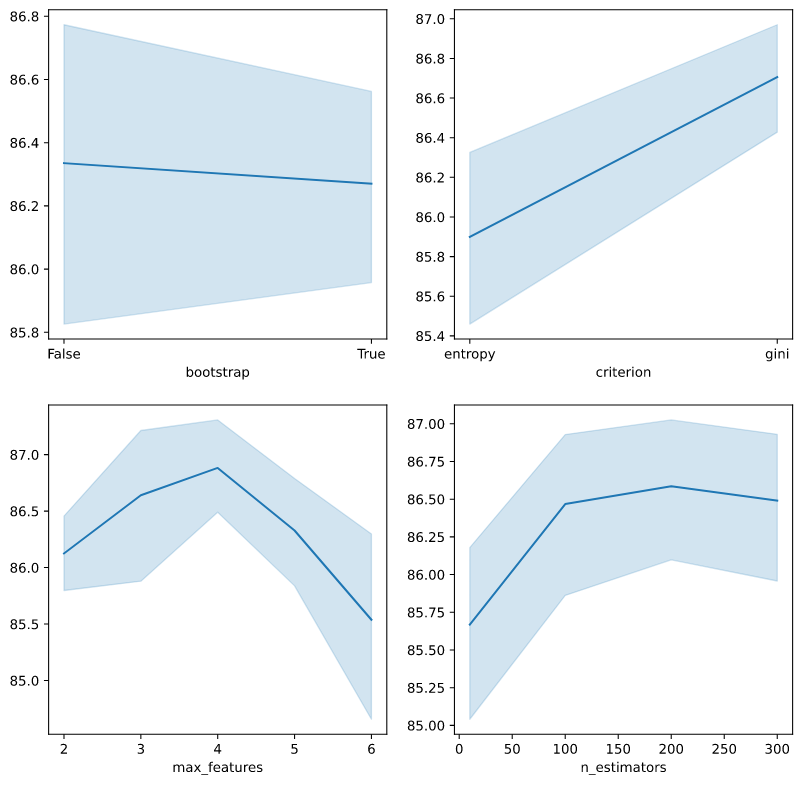
\includegraphics[width=0.5\textwidth]{figures/random_forest_parameters.png}
        \caption{\label{fig:random_forest_parameters}Résultats en fonction des paramètres}
    \end{center}
\end{figure}

On sait que le bootstrap est censé améliorer les résultats en diminuant la variance. Or le meilleur résultat est obtenu sans bootstrap. En réalité, on remarque que l'accuracy varie peu si on utilise ou pas le \textit{bootstrap}.

On distingue également une légère amélioration des résultats avec un \textit{n\_estimators} plus élevé, ce qui est logique puisque l'algorithme prend une décision à partir d'un nombre d'arbres plus élevé. Par contre cette amélioration s'arrête après un certain seuil.

Concernant le nombre de caractéristiques utilisées, on peut voir qu'on obtient une meilleur accuracy avec un \textit{max\_features} autour de 4. Cela indique qu'il y a des caractéristiques qui permettent de mieux séparer le jeu de données que d'autres.

Pour finir, on remarque une validation accuracy légèrement plus élevée pour \textit{gini}..

Il est également intéressant d'analyser l'importance de chaque caractéristique dans la prise de décision (figure~\ref{fig:random_forest_features_importance}).
En utilisant l'attribut \textit{feature\_importances\_} on remarque que \textit{degree\_spondylolisthesis} permet de classer presque la moitié des points. Cela confirme l'importance de cette variable dans la classification des individus. Par ailleurs \textit{pelvic\_radius} permet d'en séparer 20\%. Cela confirme ce qu'on pouvait voir dans la section exploration des données où la variable \textit{pelvic\_radius} semblait assez indépendante des autres, de sorte qu'elle expliquait de manière importante l'axe 2 dans l'ACP à deux dimensions (figure~\ref{fig:correlation_circle_ACP}).

\begin{figure}[htbp]
    \begin{center}
        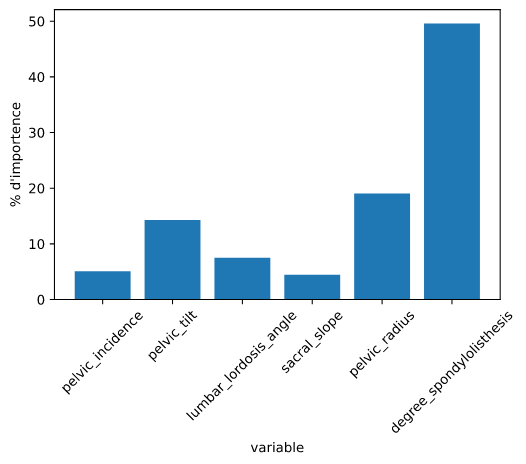
\includegraphics[width=0.45\textwidth]{figures/random_forest_features_importance.png}
        \caption{\label{fig:random_forest_features_importance}Importance des variables}
    \end{center}
\end{figure}

En appliquant le meilleur modèle à l'ensemble de test on obtient un score d'accuracy de 83.50 \%

\subsubsection{Extra Trees}
Il existe un algorithme qui pousse la randomisation encore plus loin: le \textit{Extremely randomized Trees}.
Il suit le même principe que le Random Forest. La seule différence est dans la manière de prendre une décision au niveau d'une feuille. Au lieu de choisir le meilleur seuil pour chaque caractéristique, c'est un seuil aléatoire qui est choisi.
Le meilleur seuil entre toutes les caractéristiques est ensuite choisi par le critère de séparation.
De cette manière la variance diminue encore plus, avec néanmoins un risque d'augmenter le biais\cite{scikit-learn-Extremely-Randomized-Trees}.

Nous avons donc suivi pour cet algorithme la même procédure de GridSearchCV que pour le Random Forest, avec les mêmes pré-traitements et paramètres.
On remarque une amélioration des résultats de validation pour quelques méthodes de pré-traitement, notamment pour le MinMaxScaler + NCA à deux composanates et sans \textit{pelvic\_incidence}.
On obtient un score de validation de 90.27 \% avec les paramètres suivants: \textit{bootstrap}: True,	\textit{criterion}: gini, \textit{max\_features}: 2,	\textit{n\_estimators}: 200.

Néanmoins la test accuracy baisse à 80.58 \%. On en déduit que cette méthode s'adapte mieux aux données d'apprentissage mais parvient moins bien à prédire les classes des données de test.

\section{Conclusion}

\begin{table}[htbp]
    \begin{center}
        \caption{\label{tab:accuracy_modèle}Meilleur score de test par modèle}
        \begin{tabular}{c|c}
            Modèle &  Test accuracy \\
            \hline
            QDA &  79.61 \%\\
            KNN & 81.55 \%  \\
            \textit{Régression logistique} &  \textit{84.47 \%} \\
            Random forest &  83.50 \% \\
            Extra tree &  80.58 \% \\
        \end{tabular}
    \end{center}
\end{table}

Les différentes méthodes détaillées dans ce rapport ont eu pour objectif de détecter chez des patients, des pathologies particulières. L'analyse exploratoire a mis en évidence une forte proximité entre les classes \textit{Normal} et \textit{Hernia}. Au cours de notre étude, nous avons rapidement conclu à l'inefficacité des méthodes non-supervisées au regard de notre jeu de données ce qui nous a amenés à nous concentrer sur l'apprentissage supervisé. Les différents scores de tests obtenues dans le cadre de cet apprentissage sont résumés dans le tableau \ref{tab:accuracy_modèle}. On en conclut qu'à partir de nos ensembles de tests et d'apprentissage et aux vues des variables étudiées, c'est la méthode de \textit{Régression Logistique} qui parvient le mieux à prédire l'appartenance d'un individu à une classe, sans toutefois parvenir à complètement isoler \textit{Hernia} de \textit{Normal}
 
 Plusieurs perspectives d'approfondissement peuvent toutefois être envisagées. Tout d'abord, dans le calcul du risque inhérent au choix de chacune des classes, nous avons décidé d'utiliser un coût \{0,1\} qui ne reflète pas la réalité. On pourrait augmenter le coût encouru lorsque l'on choisit la classe \textit{Normal} pour des individus ayant une hernie ou une spondylolisthesis. Sans modifier le jeu de données initial (individus et nombres de variables descriptives), il semble difficile d'obtenir des modèles beaucoup plus performants que ceux décrits précédemment. On pourrait néanmoins tenter d'appliquer la régression linéaire multiple comme méthode d'approfondissement. Celle-ci se fonde sur l'étude de la relation entre une variable à expliquer et plusieurs variables explicatives ce qui se rapproche de notre cas d'étude.
 

\appendix % la commande \appendix change la numérotation des paragraphes

\printbibliography

\end{document}
